
\begin{frame}{Tâches}
\begin{center}
\begin{tikzpicture}[mystyle]
\matrix [column sep=10mm,row sep=5mm,ampersand replacement=\&]
{
\node (i1) {\only<1-2>{X}\only<3-4>{\alert{x}}}; \&
\node [terminal] (i2) {p}; \&
\node  (i3) {\only<1>{y}\only<2>{Y}\only<3-4>{\alert{Y}}}; \\
};
\begin{scope}[every path/.style=line]
  \path (i1) -- node [left] {} (i2);
  \path (i2) -- node [right] {} (i3);
\end{scope}
\end{tikzpicture}
\end{center}
\vspace{.8cm}\only<1-3>{
\begin{description}
\item<1>[X-Y] codage, séparation de sources, extension de bande, inpainting, ...
\item<2>[X-y] recherche d'information
\item<3>[x-Y] synthèse
\end{description}}
\only<4>{
\begin{itemize}
\item attrait personnel pour l'inouï
\item challenge
\item en prise avec les avancées actuelles en apprentissage non supervisé
\end{itemize}}
\end{frame}

\begin{frame}{Requis}
\begin{description}
  \item[fidélité]: ne pas produire d'artefacts audibles
  \item[expressivité]: mécanismes de manipulation simples produisant une modification cohérente de la perception du signal résultant
  \item[versatilité]: les conditions de fidélité et d'expressivité sont remplies pour tout signal d'intérêt pour une tâche donnée
\end{description}
\end{frame}

\begin{frame}{\only<1>{Existant}\only<2>{Objectif}}
\begin{tabular}{cc}
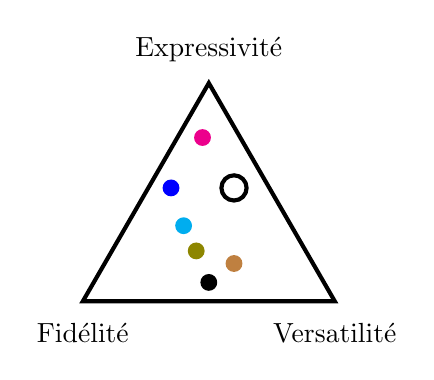
\begin{tikzpicture}[scale=0.8, label distance=1.5mm]
  \coordinate[label=below:Fidélité]  (A) at (0,0);
  \coordinate[label=below:Versatilité] (B) at (4,0);
  \coordinate[label=above:Expressivité] (C) at (2,3.464);
  \draw [line width=1.5pt] (A) -- (B) -- (C) -- cycle;
  \draw [black, fill=black, line width=1.5pt] (2,.3) circle [radius=.1 cm]; % raw
  \draw [olive, fill=olive, line width=1.5pt] (1.8,.8) circle [radius=.1 cm]; % spec
  \draw [brown, fill=brown, line width=1.5pt] (2.4,.6) circle [radius=.1 cm]; % wavelets
  \draw [cyan, fill=cyan, line width=1.5pt] (1.6,1.2) circle [radius=.1 cm]; % sct
  \draw [blue, fill=blue, line width=1.5pt] (1.4,1.8) circle [radius=.1 cm]; % slt
  \draw [magenta, fill=magenta, line width=1.5pt] (1.9,2.6) circle [radius=.1 cm]; % modal
  \only<2>{\draw [black, line width=1.5pt] (2.4,1.8) circle [radius=.2 cm];} % modal
  \end{tikzpicture}

 &

  \begin{tabular}{cl}
    \tikz\draw[black,fill=black] (0,0) circle (.1 cm); & Forme d'onde \\
    \tikz\draw[olive,fill=olive] (0,0) circle (.1 cm); & Spectrogramme \\
    \tikz\draw[brown,fill=brown] (0,0) circle (.1 cm); & Ondelettes \\
    \tikz\draw[cyan,fill=cyan] (0,0) circle (.1 cm); & Sinusoïdes à court terme \\
    \tikz\draw[blue,fill=blue] (0,0) circle (.1 cm); & Sinusoïdes à long terme \\
    \tikz\draw[magenta,fill=magenta] (0,0) circle (.1 cm); & Approches modales
  \end{tabular}
  \end{tabular}
\end{frame}

\begin{frame}{Traitement du signal pour la synthèse}
\newcommand{\blackdot}{\tikz\draw[black,fill=black] (0,0) circle (.1 cm);}
\centering
  \begin{tabular}{c|ccc}
    & fidélité & versatililité & expressivité  \\
    \hline
  multirésolution & \blackdot  & \blackdot & \\
  causalité & \blackdot  &  & \blackdot \\
  non linéarité & \blackdot  & \blackdot & \\
  dimensionalité réduite &  & &  \blackdot \\
  contrôle lent &  & &  \blackdot
  \end{tabular}
  \vspace{.5cm}
\end{frame}

\begin{frame}{Schéma fonctionnel}
  \begin{center}
  IR \\   \begin{tikzpicture}[mystyle]
      \matrix [column sep=10mm,row sep=5mm,ampersand replacement=\&]
      {
      \node (i1) {X}; \&
      \node [terminal] (i2) {$P$}; \&
      \node [terminal] (i3) {$C$}; \&
      \node (i4) {y}; \\
      };
      \begin{scope}[every path/.style=line]
        \path (i1) -- node [left] {} (i2);
      \path (i2) -- node [above] {} (i3); \path (i3) -- node [right] {} (i4);
      \end{scope}
      \end{tikzpicture}
\\ \vspace{.8cm} Synthèse \\
      \begin{tikzpicture}[mystyle]
      \matrix [column sep=10mm,row sep=5mm,ampersand replacement=\&]
      {
      \node (i1) {x}; \&
      \node [terminal] (i2) {$c$}; \&
      \node [terminal] (i3) {$P^{-1}$}; \&
      \node (i4) {Y}; \\
      };
      \begin{scope}[every path/.style=line]
        \path (i1) -- node [left] {} (i2);
      \path (i2) -- node [above] {} (i3); \path (i3) -- node [right] {} (i4);
      \end{scope}
      \end{tikzpicture}
      \end{center}
\end{frame}

\begin{frame}{Approche}
\begin{center}
 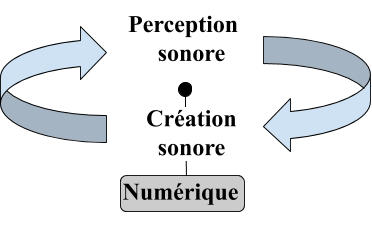
\includegraphics[width=.6\columnwidth]{longTerme}
\end{center}
\begin{description}
\item[comprendre] : mesure et qualification de l'environnement sonore et de sa perception
\item[innover] :
\begin{itemize}
\item Andy Hildebrand (Autotune)
\item Xavier Serra (Vocaloïd)
\end{itemize}
\end{description}
\end{frame}

\begin{frame}{Réseau}
\begin{block}{Local}
\begin{itemize}
\item Jean-François Petiot (LS2N)
\item Arnaud Can, Judicaël Picaut, ... (UMRAE, IFFSTAR)
\end{itemize}
\end{block}
\begin{block}{National}
\begin{itemize}
\item Nicolas Misdariis (IRCAM)
\item Catherine Lavandier (U. Cergy)
\end{itemize}
\end{block}
\begin{block}{International}
\begin{itemize}
\item Emmanouil Benetos (QMUL, UK)
\item Vincent Lostanlen (NYU, US)
\item Joakim Andèn (Flatiron Institute, US)
\end{itemize}
\end{block}
\end{frame}

\begin{frame}{Recherche à court terme}
\begin{description}
\item[ANR Cense]: inversion de descripteurs pour la synthèse de scènes sonores respectueuses de la vie privée (Félix Gontier)
\item[Ouest Industries Créatives]: conception interactive en design sonore (Tom Souaille)
\end{description}
\end{frame}

\begin{frame}{Projets à moyen terme}
\begin{itemize}
\item inversion de l'opérateur de diffusion d'ondelettes
\item synthèse audio neuronale
\item en particulier les approches basées échantillons
\end{itemize}
\end{frame}

\begin{frame}{Déplacements US}
\begin{block}{Côte ouest}
\begin{itemize}
\item \structure{Jesse Engel}, magenta, Google brain (SFB)
\item Justin Salamon, audio research group, Adobe research (SFB)
\end{itemize}
\end{block}
\begin{block}{Côte est}
\begin{itemize}
\item Juan Pablo Bello, music and audio research group, NYU (NY)
\item Mounya Elhilali, Laboratory for Computational Audio Perception, Johns Hopkins University (Baltimore)
\end{itemize}
\end{block}
\end{frame}

\begin{frame}{Contributions}
\small
Publications
\begin{itemize}
\item \fullcite{lagrangeTaslp06}
\item \fullcite{lagrangeTaslp08}
\item \fullcite{lafayhal-01111381}
\end{itemize}
Logiciels
\begin{itemize}
\item \fullcite{explanes}
\item \fullcite{simscene}
\end{itemize}
\end{frame}
